\newpage

\section*{ $^{115}$In(n,$\gamma$)$^{115}$In }

Power Level: 100 kW(th) \\
Time at Power: 30 s \\
Wait Time: 7200 s \\
Total Activity at Removal: 9.81e+03 $\mu Ci$

\begin{table*}[h]
\centering
\begin{tabular}{ |c|c|c|c|c|c| }
 \hline
 Position & Mass $mg$ & Counting Time $s$ & Counting Activity $\mu Ci$ & Expected Area (Counts) \\
 \hline 
 1 & 6.6000000000000005 & 60 & 4.37e+02 & 1.27e+07\\ 
\hline
 2 & 6.6000000000000005 & 60 & 7.04e+02 & 2.05e+07\\ 
\hline
 3 & 6.6000000000000005 & 60 & 6.27e+02 & 1.83e+07\\ 
\hline
 4 & 6.6000000000000005 & 60 & 3.18e+02 & 9.26e+06\\ 
\hline
\end{tabular}
\end{table*}

\begin{figure}[!ht]
   \centering
   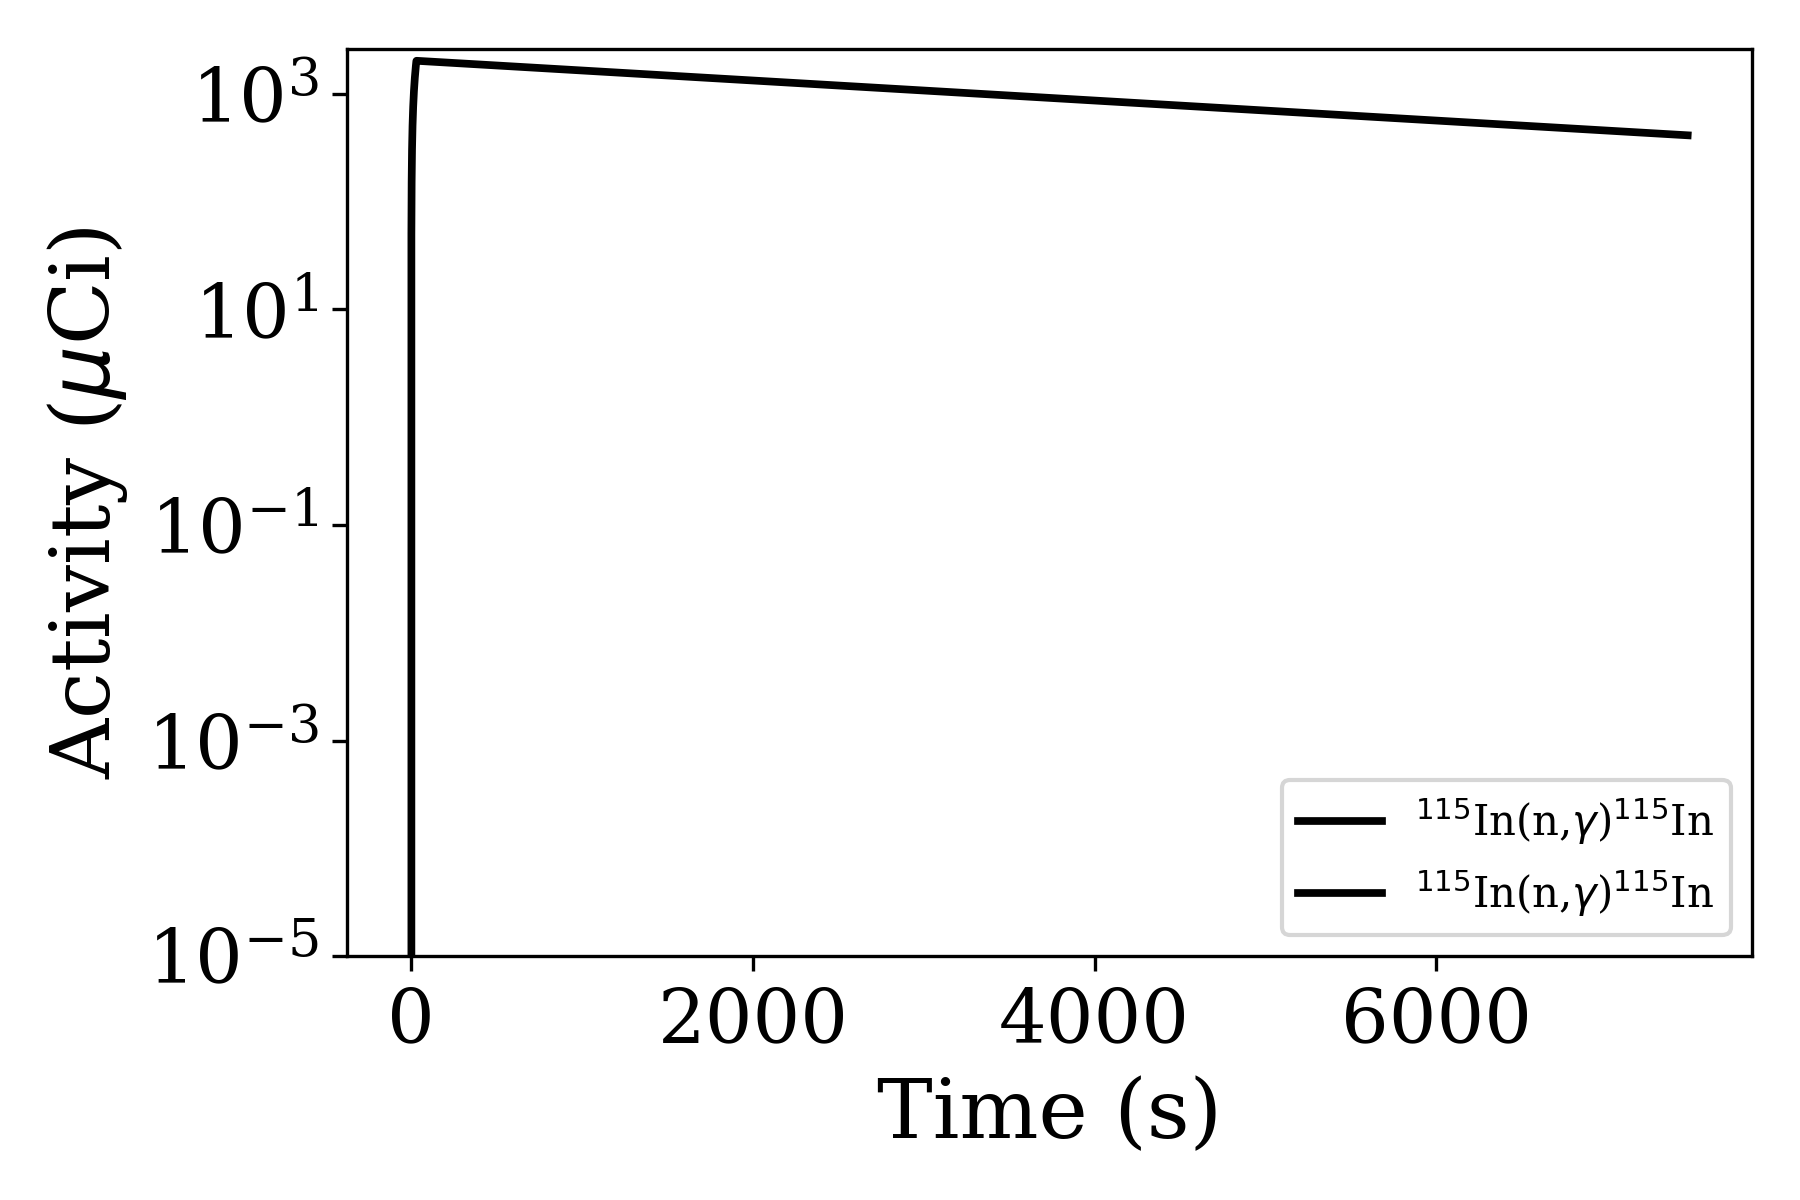
\includegraphics[width=.4\textwidth]{source/plot/In-115(n,gamma)In-116_wisconsin1.png} 

\end{figure}

\begin{figure}[!ht]
   \centering
   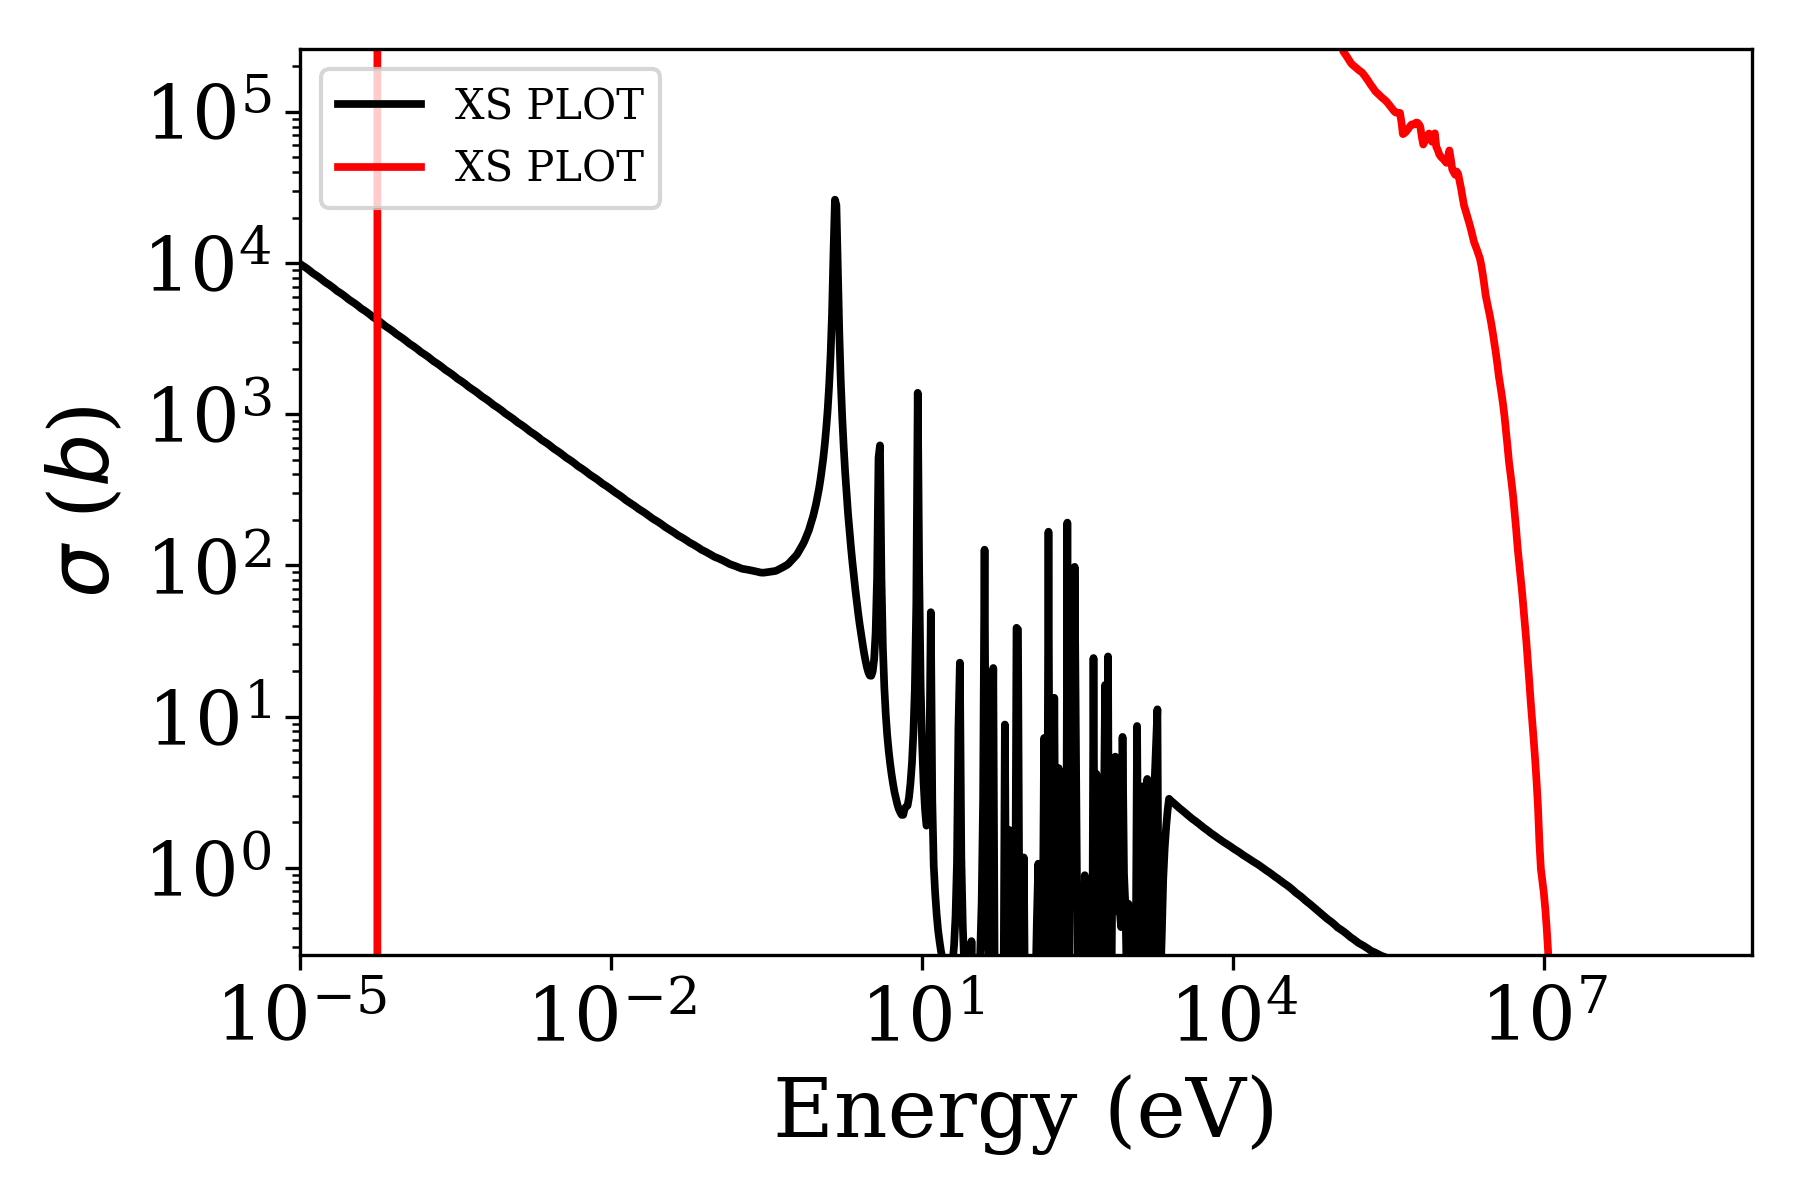
\includegraphics[width=.4\textwidth]{source/plot/In-115(n,gamma)In-116.png} 

\end{figure}

\begin{table*}[h]
\centering
\begin{tabular}{ |c|c|c|c|c|c|c| }
 \hline
 Reaction & T$_{1/2}$ & ROI (eV) & Important Gammas (keV) \\
 \hline 
 $^{115}$In(n,$\gamma$)$^{115}$In & 54.0 m & 1.41e-02, 1.63e+00 & 1293(0.8),  \\ 
\hline
\end{tabular}
\end{table*}
